\chapter{First Law of Thermodynamics}
\begin{itemize}
    \begin{table}[H]
        \centering
        \begin{tabular}{M{0.2\textwidth}M{0.4\textwidth}M{0.4\textwidth}}
            \toprule
            Difference & Evaporation & Boiling\\
            \midrule
            Temperature & Occurs at all temperatures & At each pressure, there is exactly one fixed temperature at which boiling occurs.\\
            \midrule
            Location & Occurs only at the surface of a liquid & Occurs throughout the liquid\\
            \bottomrule
        \end{tabular}
        \caption{Differences between evaporation and boiling.}
        \label{table:evaporation-vs-boiling}
    \end{table}
    \item The \emph{heat capacity} of a body is defined as the amount of thermal energy required to raise its temperature by one Kelvin / degree Celsius. 
    \item The specific \emph{heat capacity} of a body is defined as the amount of thermal energy required to raise the temperature of one unit mass of the substance by one Kelvin / degree Celsius.
    \item For a substance of mass \(m\), heat capacity \(C\), and specific heat capacity \(c\), we write \(Q=C\Delta\theta=mc\Delta\theta\).
    \item \emph{Note.} In the case that the mass of gas present is not explicitly given, check whether the question specified what the gas is. For example, there might have been a sneaky mention that the gas is neon-20, so \(m=20N\) unified atomic masses can be deduced 
    \item The \emph{specific latent heat} of a body is defined as the thermal energy required to change \emph{phase} of one unit mass of a substance, \emph{without a change in temperature}.
    \item For a substance of specific latent heat of fusion (vaporisation), we write \(Q=mL_f\) (\(Q=mL_v\)).
    \item \emph{Internal energy} of a system is a sum of \emph{random distribution} of kinetic and potential energies \emph{associated with the molecules} of the system. Microscopic potential energy is due to the intermolecular forces between the molecules. Microscopic kinetic energy is due to the random motion of the molecules. 
    \item The \emph{internal energy of an ideal gas} is the sum of microscopic kinetic energies due to the random motion of the ideal gas molecules. 

    \emph{Note.} The inclusion of microscopic potential energy is forbidden, since ideal gases have zero microscopic potential energy.
    \item Words such as ``insulated'' implies that there is no heat supplied to the system. i.e. \(Q=0\).
    \item \emph{Note.} Work done versus heat supplied. Work done is the transfer of energy by force/macroscopic changes, while heat supplied is the direct transfer of thermal energy through microscopic changes. E.g. consider a liquid that is isolated from all other sources of heat. When stirring leads to an increase in temperature (via frictional heating), it is considered work done, even though the liquid experiences an increase in thermal energy.
    \item An ideal monoatomic gas of \(N\) atoms only has translational motion and no intermolecular potential energy, \(U=E_k=N\cdot\text{translational \(E_k\) of one atom}=\frac{3}{2}NkT\).
    \item For non-monoatomic ideal gases, \(U\neq \frac{3}{2}NkT\). But we know that \(U_{\text{Total}}\propto NT\) and \(U_{\text{one molecule}}\propto T\).
    \item The \emph{First Law of Thermodynamics} states that the \emph{increase} in internal energy of a closed system is the \emph{sum} of heat \emph{supplied} to the system and the work done \emph{on} the system. i.e. \(\Delta U=Q+W\).
    \item The work done \(W\) on a gas against a constant external pressure \(p\) is such that \(W=-p\Delta V\).
    \item In general, the work done on a gas is \(W=-\int_{V_i}^{V_f}p\,dV\).
    \item An \emph{\textcolor{blue}{isothermal} process} is one that takes place without a change in temperature, i.e. \(\Delta T=0\). Thus, for an ideal gas (possibly non-monoatomic), \(\Delta U=0\) since \(U\propto T\).
    \item An \emph{\textcolor{pink!75!red}{iso-volumetric/isochoric} process} is one that takes place without a change in volume, i.e. \(\Delta V=0\). Hence, when the external pressure is constant, \(W=0\).  
    \item An \emph{\textcolor{green!85!black}{isobaric} process} is one that takes place without a change in pressure, i.e. \(\Delta p=0\).
    \item An \emph{\textcolor{red!60!black}{adiabatic} process} is one that takes place without heat transfer, i.e. \(Q=0\). Therefore, \(U=W\).
    \begin{figure}[H]
        \centering
        \begin{subfigure}[c]{0.30\textwidth}
            \centering
            \includegraphics[page=6]{../images/Thermodynamics/Thermodynamics.pdf}
            \caption{An \textcolor{blue}{isothermal} process.}
            \label{fig:isothermal}
        \end{subfigure}%
        \begin{subfigure}[c]{0.30\textwidth}
            \centering
            \includegraphics[page=7]{../images/Thermodynamics/Thermodynamics.pdf}
            \caption{\textcolor{pink!75!red}{Iso-volumetric} and \textcolor{green!85!black}{isobaric} processes.}
            \label{fig:iso-volumetric}
        \end{subfigure}%
        \begin{subfigure}[c]{0.30\textwidth}
            \centering
            \includegraphics[page=8]{../images/Thermodynamics/Thermodynamics.pdf}
            \caption{An An \textcolor{red!60!black}{adiabatic} process.}
            \label{fig:adiabatic}
        \end{subfigure}%
        \caption{\ref{source:thermodynamic-processes} Illustrations for isothermal, iso-volumetric/isochoric, isobaric, and adiabatic processes.}
        \label{fig:thermodynamic-processes-PV-diagram}
    \end{figure}
    \item A thermodynamic cyclic process is one that eventually returns to its initial state. 
    \begin{itemize}
        \item \(\Delta U=0\) so \(Q=-W\). 
        \item The net work done by/on the gas is given by the area enclosed by the closed loop.
    \end{itemize}
    \begin{figure}[H]
        \centering
        \begin{subfigure}[c]{0.30\textwidth}
            \centering
            \includegraphics[page=4]{../images/Thermodynamics/Thermodynamics.pdf}
            \caption{A simple engine.}
            \label{fig:simple-engine-theromdynamics-closed-loop}
        \end{subfigure}%
        \begin{subfigure}[c]{0.30\textwidth}
            \centering
            \includegraphics[page=10]{../images/Thermodynamics/Thermodynamics.pdf}
            \caption{An Otto cycle}
            \label{fig:otto-cycle-theromdynamics-closed-loop}
        \end{subfigure}%
        \begin{subfigure}[c]{0.30\textwidth}
            \centering
            \includegraphics[page=11]{../images/Thermodynamics/Thermodynamics.pdf}
            \caption{A Carnot cycle.}
            \label{fig:carnot-cycle-theromdynamics-closed-loop}
        \end{subfigure}%
        \caption{\ref{source:thermodynamic-processes} Some thermodynamic cyclic processes.}
        \label{fig:thermodynamic-cyclic-processes}
    \end{figure}
\end{itemize}